\begin{figure}
\centering

\begin{subfigure}{\columnwidth}
  \centering
  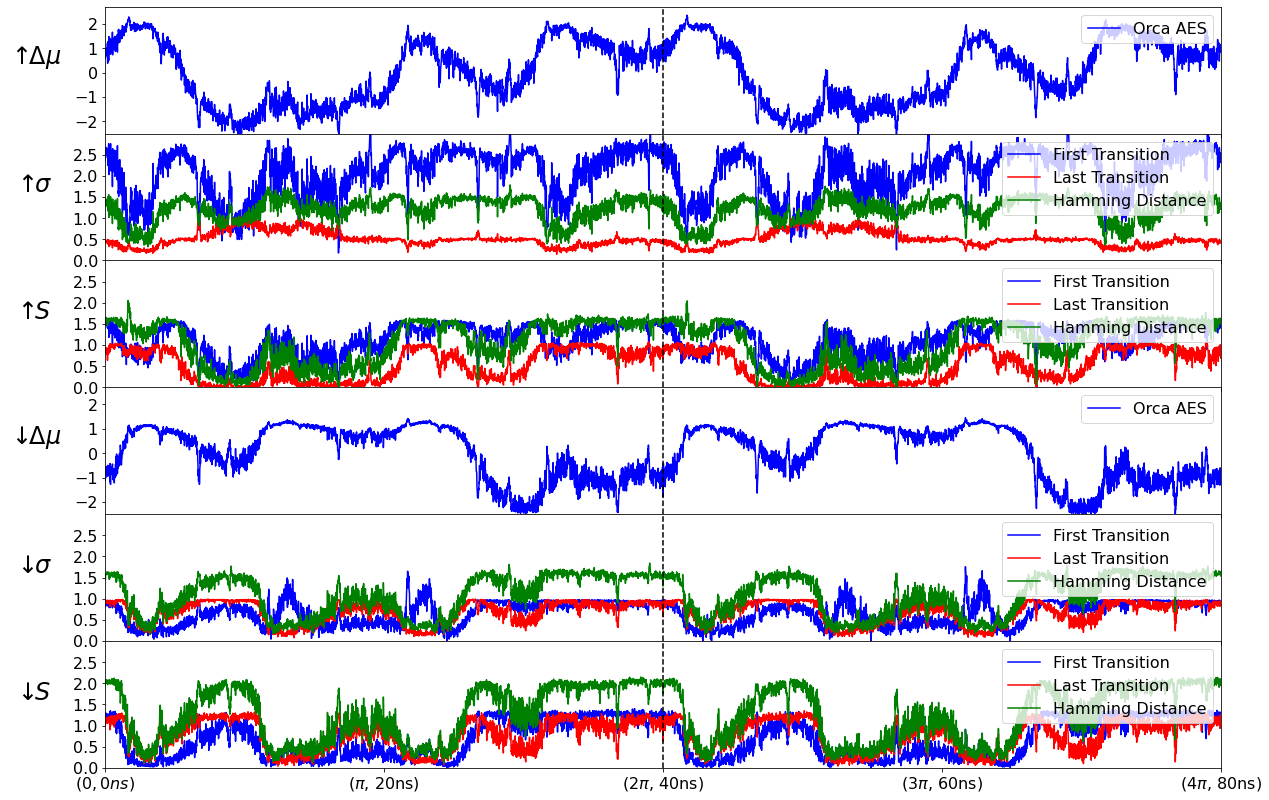
\includegraphics[width=\linewidth]{img/orca_aes_phi_entropy_std_metric.png}
  %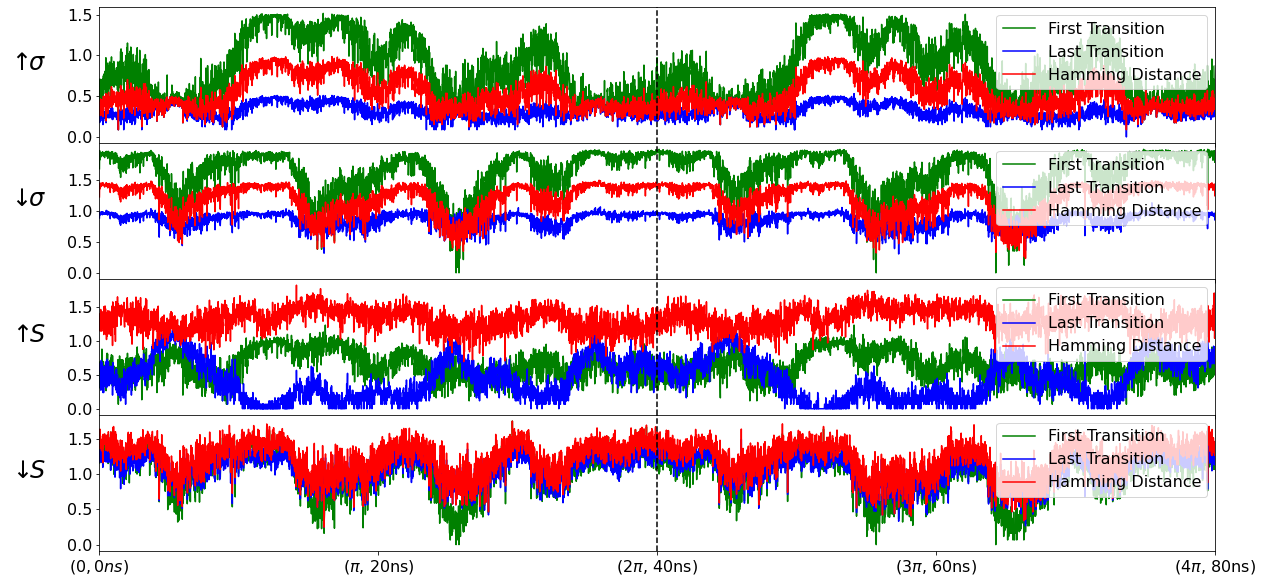
\includegraphics[width=\linewidth]{img/pico_aes_phi_entropy_std_metric.png}

%  \caption{First Index Entropy by $\phi$}
  %\label{fig}
\end{subfigure}

%\begin{subfigure}{\columnwidth}
%  \centering
%  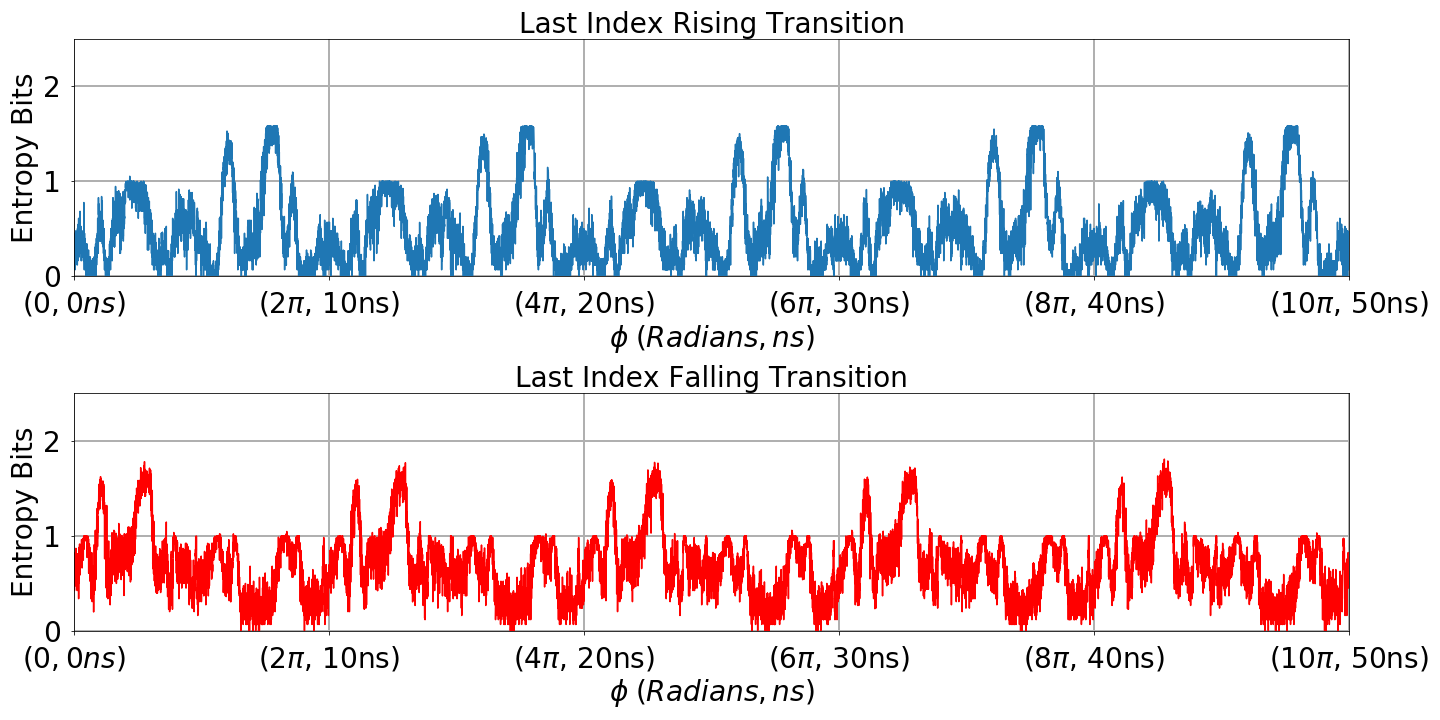
\includegraphics[width=\linewidth]{img/last_entropy_orca.png}
%  \caption{Last Index Entropy by $\phi$}
%  %\label{fig}
%\end{subfigure}

%\bigskip

%\begin{subfigure}{\columnwidth}
%  \centering
%  \includegraphics[width=\linewidth]{img/hamming_entropy_orca.png}
%  \caption{Hamming Distance Entropy by $\phi$}
%\end{subfigure}
%\bigskip


%\begin{subfigure}{\columnwidth}
%  \centering
%  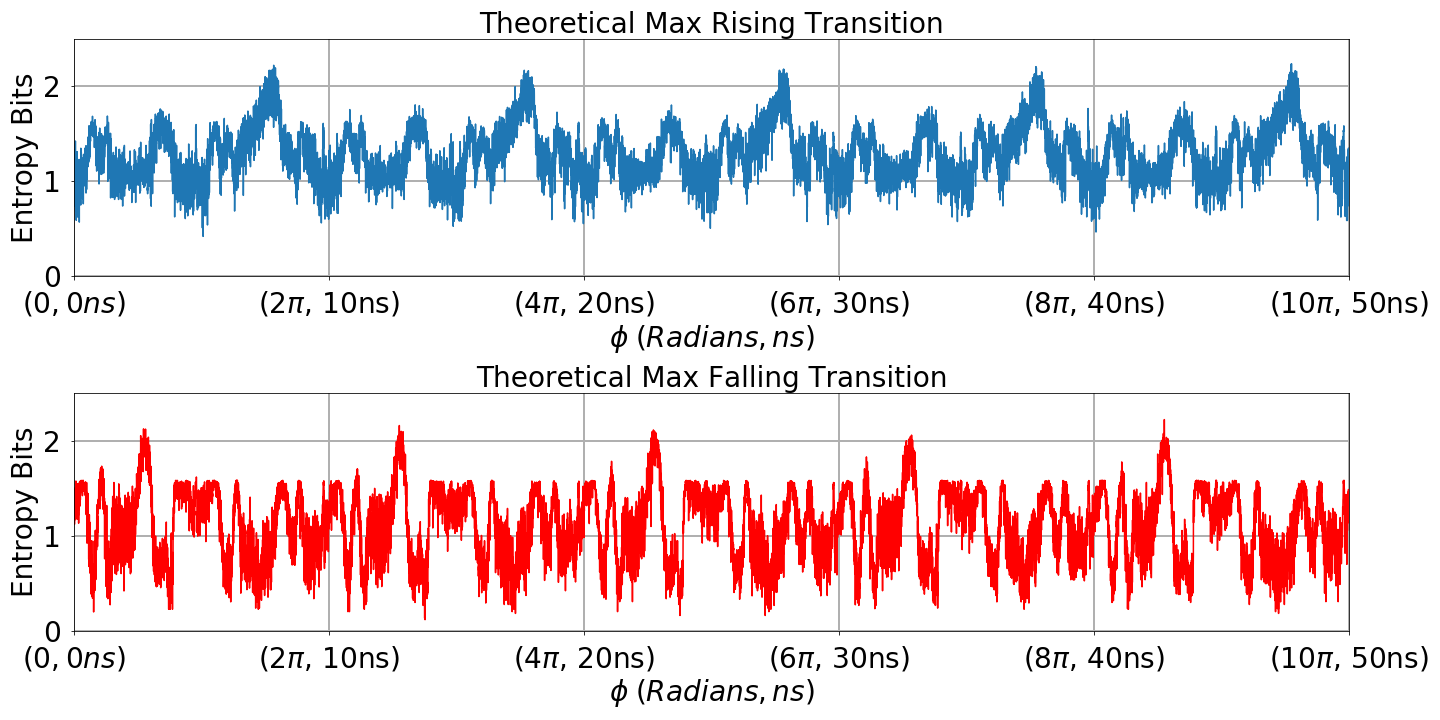
\includegraphics[width=\linewidth]{img/max_entropy_orca.png}
%  \caption{Theoretical Maximum Entropy by $\phi$ \cd{describe binary to int method and why it is the max possible}}
 % \label{fig:}
%\end{subfigure}
\caption{Channel information measured by the sensor as $\phi$ is swept from 0 to 4$\pi$ while the ORCA-AES target computation is running.
We plot the Binary Hamming Distance deviation from the mean for the rising  ($\uparrow\Delta\mu$) and falling transition $\downarrow\Delta\mu$), the standard deviation, for the rising ($\uparrow\sigma$) and falling transition ($\downarrow\sigma$), and the the entropy for rising ($\uparrow S$) and falling transition ($\downarrow S$). The entropy is a measure of information measured by the sensor and the entropy is maximized by the falling transition with the \textit{Binary Hamming Distance} metric. The standard deviation is well correlated with entropy, and a simpler computation, so we use when tuning our sensor in Section~\ref{channel_capacity}.
%\dr{fix reference, remove background from 1/4}.
}

\label{fig:orca-entropy}
\end{figure} 
